\documentclass[11pt]{article}

% --- arXiv-safe preamble --------------------------------------------------
\usepackage[utf8]{inputenc}
\usepackage[T1]{fontenc}
\usepackage{lmodern}
\usepackage{amsmath,amssymb}
\usepackage{graphicx}
\usepackage{booktabs}
\usepackage{array}
\usepackage{microtype}
\usepackage{authblk}
\usepackage{caption}
\usepackage[numbers,sort&compress]{natbib}
\usepackage[hidelinks]{hyperref}

\graphicspath{{figures/}}

% degree symbol that works in text and math, no extra package needed
\newcommand{\dgr}{\ensuremath{^{\circ}}}
\newcommand{\sigavg}{\ensuremath{\sigma_{\text{avg}}}}

\title{SamSeesSheep: A Measurement Pipeline for Sheep Ear-Angle
Extraction from Ambient Pasture Video Using Foundation-Model Annotation}

\author[1]{Antone King}
\affil[1]{Lorewood Labs, Middletown, Delaware, USA \\ \texttt{antone@lorewood.dev}}
\date{}

\begin{document}
\maketitle

\begin{abstract}
The Sheep Pain Facial Expression Scale (SPFES) \citep{mclennan2019} requires
trained human observers to score pain frame-by-frame from video, a bottleneck
that limits the scale and reproducibility of ovine welfare research. No
automated system currently exists to extract the relevant ear-angle
measurements from ambient pasture video. I present SamSeesSheep, a measurement
pipeline that uses a foundation video segmentation model (SAM~3 Video) as an
annotation tool, a human-in-the-loop review interface, and a lightweight
edge-runnable keypoint detector (YOLO-pose, 2.5\,M parameters, ${\sim}10$\,MB)
trained on the reviewed output. The pipeline produces per-keypoint residual
standard-deviation benchmarks on genuinely held-out clips. On a clip never seen
by the labeler or trainer, v0.4 achieves $\sigma = 4.06\dgr$ (left ear) and
$4.09\dgr$ (right ear) for ear angle. On a second, independently selected
held-out clip with a different flock arrangement and lighting, v0.7 reaches
$\sigavg = 2.84\dgr$ (left $2.39\dgr$, right $3.29\dgr$); the difference between
the two clips reflects clip characteristics rather than a model improvement
(on matched clips, v0.7 and v0.4 are statistically indistinguishable). Both
ear-angle metrics are derived from five head keypoints (nose, left/right ear
bases, left/right ear tips). Stock YOLO (\texttt{yolo26n.pt}) produces zero
keypoints on both clips. The training progression from 98 to 405 reviewed
instances across 3 to 8 training videos shows monotonically improving keypoint
stability; beyond that, through 523 instances and 11 videos (v0.7), stability
plateaus at the clip noise floor, with a documented per-keypoint regression at
v0.6. I explicitly do not claim pain detection or welfare scoring; the pipeline
is a measurement instrument designed to lower the data-collection barrier for
researchers who need reproducible ear-angle features from ambient footage.
\end{abstract}

\begin{figure}[t]
  \centering
  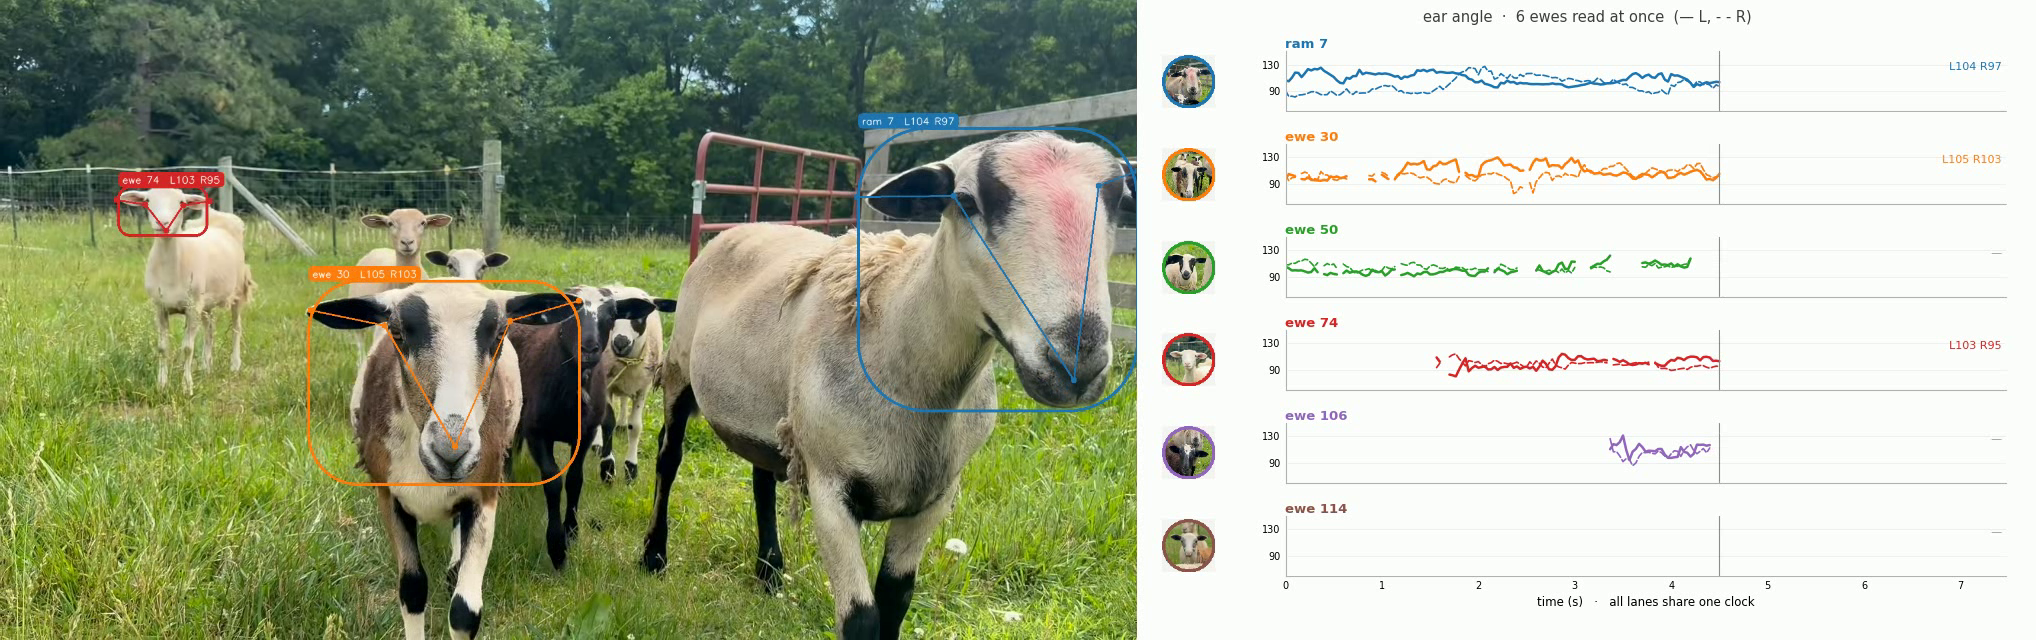
\includegraphics[width=\textwidth]{hero.png}
  \caption{SamSeesSheep pipeline output on held-out clip HO-2
  (Table~\ref{tab:clipmap}): simultaneous ear-angle monitoring of six animals. \emph{Left:} the
  supervision-annotated flock with bounding boxes, per-animal labels (including
  left/right ear angles in degrees), and five-keypoint skeletons (nose, ear
  bases, ear tips). \emph{Right:} a six-lane synchronized ear-angle chart with
  dual traces per lane (solid = left ear, dashed = right ear) and per-animal
  thumbnails. The frame is a still extracted from the rendered video
  \texttt{synced-lanes-6ewes-pro-Test\_Clip\_Morning.mp4} (2036$\times$640\,px,
  7.5\,s; see Data Availability). The figure demonstrates the pipeline's
  end-to-end path: ambient pasture video $\rightarrow$ foundation-model
  annotation $\rightarrow$ human review $\rightarrow$ multi-animal time-series
  ear-angle extraction, running on an edge GPU with a ${\sim}10$\,MB model.}
  \label{fig:hero}
\end{figure}

\section{Introduction}

Sheep welfare assessment has advanced through the development of facial
expression scales. The Sheep Pain Facial Expression Scale (SPFES), validated by
McLennan and Mahmoud \citep{mclennan2019}, identifies five facial action units,
including ear posture, that correlate with pain states in clinical conditions
such as foot rot, mastitis, and post-surgical recovery. Ear posture in
particular has been established as an indicator of emotional valence in sheep by
multiple independent groups \citep{reefmann2009,boissy2011}. The SPFES protocol,
however, requires trained human observers to score each frame of video
manually. For a single 30-second clip at even a modest frame rate, this is
hundreds of individual scoring decisions. Scaling to continuous monitoring
across multiple animals and days is operationally infeasible without
automation.

The gap is not in the biological validity of ear-angle features; it is in the
measurement infrastructure. No automated system extracts ear-angle measurements
from ambient pasture video with quantified, reproducible accuracy. Building one
requires solving a sequence of practical computer-vision problems: detecting
sheep heads in unconstrained outdoor conditions, localizing five anatomical
keypoints per head (nose, left/right ear bases, left/right ear tips), tracking
them across frames, and deriving a stable ear-angle signal from the keypoint
geometry. Off-the-shelf object detectors provide sheep bounding boxes on
roughly a third of frames but produce no landmark keypoints; the ear-angle
signal is literally unmeasurable without a custom-trained keypoint head.

Foundation models have changed the economics of annotation. SAM~3 Video
\citep{ravi2025sam3}, prompted with plain-English phrases (``sheep head,''
``sheep ear,'' ``sheep nose''), can segment every sheep in a clip and track
them across frames. This converts the labeling task from creation (drawing
boxes and placing landmarks from scratch on every frame) to review (confirming
or correcting machine-generated candidates). A domain expert who knows what a
sheep's ear looks like, but who is not a machine-learning engineer, can produce
a reviewed keypoint dataset in hours rather than weeks.

I exploit this transformation to build a measurement pipeline: SAM~3 Video
auto-segments sheep in short phone-captured clips; a labeling UI presents
machine-generated keypoint candidates for human review; reviewed frames export
to a YOLO-pose dataset; a small model (YOLO26n-pose, 2.5\,M parameters) trains
on a cloud GPU; and the resulting weights (${\sim}10$\,MB) run inference on a
consumer-grade edge GPU (6\,GB). The pipeline produces per-keypoint residual
standard-deviation ($\sigma$) benchmarks on genuinely held-out clips, evaluated
against a stock-YOLO baseline that produces zero keypoints.

\paragraph{Contributions.}
\begin{enumerate}
  \item A complete, open-source pipeline that converts ambient pasture video
  into a reviewed sheep-head keypoint dataset using a foundation model as the
  annotation engine and a human as the reviewer.
  \item A trained edge-runnable keypoint detector (YOLO26n-pose, 2.5\,M
  parameters, ${\sim}10$\,MB) that places five keypoints on every detected sheep
  head, achieving ${\sim}4\dgr$ ear-angle $\sigma$ on a held-out clip.
  \item A reproducible benchmark protocol using genuinely held-out clips with
  per-keypoint residual $\sigma$, derived ear-angle $\sigma$, bootstrap
  confidence intervals, and a stock-YOLO baseline. The protocol is applied to
  two independent held-out clips (HO-1 and HO-2; Table~\ref{tab:clipmap})
  spanning different flock arrangements, lighting,
  and model versions.
  \item A documented training progression (v0.2 $\rightarrow$ v0.7). Keypoint
  stability improves monotonically from 98 to 405 reviewed instances (3 to 8
  videos, v0.2 $\rightarrow$ v0.4); beyond that it plateaus at the clip noise
  floor, and the progression includes a regression case (v0.6) that isolates
  per-keypoint labeling consistency from raw instance count. v0.7 reaches
  $\sigavg = 2.84\dgr$ on the second held-out clip; this is a noise-floor
  measurement on a different clip, not an improvement over v0.4 (Section
  \ref{sec:crossclip}).
  \item A measurement instrument --- not a pain detector, not a welfare scorer
  --- designed to reduce the data-collection barrier for researchers who need
  reproducible ear-angle features from ambient pasture footage.
\end{enumerate}

I am explicit about what this work is not. It is not a pain detection system. It
is not a welfare assessment tool. It has not been validated against documented
stress events. It runs on a single Katahdin flock on one farm in Delaware, USA,
with one smartphone camera, annotated by a single non-veterinarian operator.
Generalization to other breeds, flocks, geographies, or clinical contexts is
future work requiring independent validation. This paper describes a measurement
instrument that extracts ear-angle features with quantified stability, and the
pipeline that built it.

\section{Related Work}

\subsection{Ovine Facial Expression Scales and Ear Posture}
McLennan and Mahmoud \citep{mclennan2019} developed the SPFES, identifying five
facial action units --- orbital tightening, cheek tightening, ear posture, lip
and jaw tension, and nostril and philtrum shape --- that trained observers score
to assess pain in sheep. Their automated SPFES system used hand-crafted features
and required manually annotated facial landmarks. The ear-posture unit
classifies ear position into three categories (forward/alert, neutral,
backward/flattened), with backward posture a strong pain indicator. Reefmann et
al.\ \citep{reefmann2009} and Boissy et al.\ \citep{boissy2011} independently
established ear postures as indicators of emotional valence, finding that
asymmetric or backward positions correlate with negative affective states.
These studies provide the biological grounding for ear-angle measurement but
rely on trained human observers for frame-by-frame scoring. The gap we address
is the absence of an automated measurement pipeline.

\subsection{Foundation Models for Agriculture}
The Segment Anything Model family \citep{kirillov2023segment,ravi2024sam2,ravi2025sam3}
has demonstrated strong zero-shot segmentation. SAM~3 Video extends this to the
temporal domain, tracking objects across frames from text or click prompts. In
agriculture, foundation models have been applied to crop monitoring, weed
detection, and livestock identification \citep{li2024foundation}. Most such work
uses foundation models for direct inference; our pipeline inverts this --- SAM~3
Video is the annotation backbone that produces the labeled data training a
lightweight deployment model.

\subsection{Keypoint Detection and YOLO-Pose}
YOLO-pose \citep{maji2022yolopose} extends YOLO object detection with a keypoint
regression head, enabling simultaneous box detection and keypoint localization
in one forward pass. The YOLO26n-pose variant (2.5\,M parameters) suits edge
deployment within consumer-GPU memory. Keypoint detection has been applied to
animal pose estimation in laboratory and controlled-farm settings
\citep{mathis2018deeplabcut,graving2019deepposekit,pereira2022sleap}, but those
tools assume manual annotation workflows or controlled capture. This work targets
ambient, unconstrained pasture video with a foundation-model-assisted annotation
pipeline.

\subsection{Precision Livestock Farming}
PLF systems \citep{berckmans2014precision} use sensors and computer vision for
continuous monitoring, targeting metrics such as feeding behavior, locomotion,
and social interaction. Commercial platforms operate at enterprise scale with
proprietary models. This work occupies a different niche: an open-source,
solo-operator-scale pipeline demonstrating the feasibility of building a
domain-specific keypoint detector from scratch using foundation-model
annotation, with explicit quantification of measurement stability.

\subsection{The Gap}
No existing system provides an end-to-end pipeline that (a) uses a foundation
model for automated sheep-head keypoint annotation, (b) incorporates a
human-in-the-loop review step, (c) exports a standard-format dataset for
training an edge-runnable model, and (d) publishes reproducible held-out
benchmarks with per-keypoint $\sigma$, derived ear-angle $\sigma$, and a
stock-model baseline. This is the gap I fill.

\section{Method}

\subsection{Pipeline Overview}
The pipeline consists of five stages connected by well-defined data-format
contracts, summarized in Figure~\ref{fig:pipeline}.

\begin{figure}[t]
  \centering
  \fbox{\begin{minipage}{0.92\textwidth}
  \small\ttfamily
  Phone capture (1080p, 15--30 s, .MOV)\\
  \phantom{xx}$\rightarrow$ Frame extraction (2 fps, ${\sim}512$ px max dimension)\\
  \phantom{xxxx}$\rightarrow$ SAM~3 Video text-prompted segmentation\\
  \phantom{xxxxxx}$\rightarrow$ Keypoint derivation from masks\\
  \phantom{xxxxxxxx}$\rightarrow$ Human review in labeling UI\\
  \phantom{xxxxxxxxxx}$\rightarrow$ YOLO-pose dataset export\\
  \phantom{xxxxxxxxxxxx}$\rightarrow$ Cloud GPU training (RTX 4090, ${\sim}6$ min)\\
  \phantom{xxxxxxxxxxxxxx}$\rightarrow$ Edge inference + $\sigma$ benchmark (GTX 1660 Ti, 6 GB)
  \end{minipage}}
  \caption{The five-stage SamSeesSheep pipeline. Only the trained weights cross
  from cloud to edge; the dataset remains on the training host.}
  \label{fig:pipeline}
\end{figure}

\subsection{Video Capture and Frame Extraction}
Clips are captured at 1080p, 30\,fps, typically 15--30\,s. Frames are extracted
at 2\,fps using PyAV with a maximum dimension of 512\,px (aspect-ratio
preserved). The 2\,fps rate and 512\,px resolution keep SAM~3 Video within GPU
memory budget (24\,GB for the full three-session pipeline; 6\,GB for the reduced
two-session variant) while providing sufficient temporal resolution for the
sheep-head labeling task, where head pose changes slowly.

\subsection{SAM~3 Video Segmentation and Keypoint Derivation}
SAM~3 Video (\texttt{facebook/sam3} on Hugging Face, ${\sim}3$\,GB) is called
with three text prompts, each a separate propagation session: ``sheep head''
$\rightarrow$ head mask; ``sheep ear'' $\rightarrow$ left/right ear masks;
``sheep nose'' $\rightarrow$ nose mask. The nose session requires a 24\,GB GPU;
on a 6\,GB GPU the pipeline drops to two sessions (head + ear) and nose
keypoints fall back to head-mask geometry. SAM~3's internal tracker handles
multiple instances natively. From the masks, five keypoint candidates are
derived per instance per frame (Table~\ref{tab:kpts}). Keypoints are stored in
image-space pixel coordinates; left/right is from the camera's perspective. Each
keypoint carries a visibility flag $v$: $v{=}0$ (absent), $v{=}1$ (auto-placed,
unreviewed), $v{=}2$ (human-reviewed).

\begin{table}[t]
  \centering
  \caption{Keypoint slots and their derivation from SAM~3 masks.}
  \label{tab:kpts}
  \begin{tabular}{cll}
    \toprule
    Slot & Name & Derivation \\
    \midrule
    0 & Nose tip & Centroid of nose mask, or anterior point of head mask when no nose mask \\
    1 & Left ear base & Point on left ear mask closest to head-mask centroid \\
    2 & Right ear base & Point on right ear mask closest to head-mask centroid \\
    3 & Left ear tip & Point on left ear mask farthest from head-mask centroid \\
    4 & Right ear tip & Point on right ear mask farthest from head-mask centroid \\
    \bottomrule
  \end{tabular}
\end{table}

\subsection{Labeling UI and Review Protocol}
The interface is a FastAPI backend serving a vanilla-JavaScript frontend. For
each frame the reviewer sees SAM~3-derived candidates overlaid on the source
image: \texttt{A} accepts all keypoints for the current instance, dragging a dot
corrects placement, \texttt{Enter} saves and advances. The schema supports
multi-instance frames. A single operator (the author, not a veterinarian)
performed all reviews; each video was reviewed in a single session. An instance
with any $v{=}2$ keypoint counts as ``reviewed''; all five at $v{=}2$ is ``fully
reviewed.''

\subsection{YOLO-Pose Export and Training}
Only $v{=}2$ keypoints enter the dataset. Export produces YOLO-pose format: one
\texttt{.txt} per image, one line per instance, class index 0
(\texttt{sheep\_head}), normalized box, and five normalized keypoint triples
$(x,y,v)$. The \texttt{data.yaml} declares \texttt{kpt\_shape: [5, 3]} and
\texttt{flip\_idx: [0, 2, 1, 4, 3]}, so horizontal-flip augmentation correctly
swaps left/right ear keypoints. The train/val split uses deterministic MD5 hash
bucketing per \texttt{(video\_id, frame\_idx)}: frames with
$\text{bucket} < 0.2$ go to validation. The split is per-frame (not per-video),
appropriate for a single-flock, single-camera scope where generalization to
unseen poses from known scenes is the target. Training uses YOLO26n-pose (2.5\,M
parameters), 100 epochs, batch 8, image size 640, on an RTX 4090 via RunPod;
training completes in ${\sim}6$ minutes and \texttt{best.pt} is ${\sim}10$\,MB.

\subsection{Edge Inference and Benchmark Protocol}
\label{sec:bench}
Inference runs on a local GTX 1660 Ti (6\,GB). The protocol, implemented in
\texttt{sheep-yolo/scripts/bench\_held\_out.py}, evaluates keypoint stability on
a genuinely held-out clip:
\begin{enumerate}
  \item \textbf{Clip selection.} A clip with low similarity to every training
  video (see Data Availability for the screening procedure) and never pushed to
  the labeler.
  \item \textbf{Target window.} A ${\sim}5$\,s segment where a target sheep's
  head is approximately stationary; an ROI filter excludes neighbouring sheep.
  \item \textbf{Residual $\sigma$.}
  $\sigma_{\text{residual}} = \mathrm{std}\!\left(\text{kpt} -
  \mathrm{median}_7(\text{kpt})\right)$. The 7-frame rolling median strips slow
  head drift (the sheep's actual motion) and isolates frame-to-frame jitter.
  \item \textbf{Raw $\sigma$.} $\mathrm{std}(\text{kpt})$ over the window,
  dominated by head sway; a sanity check that all models track the same physical
  motion.
  \item \textbf{Ear-angle $\sigma$.} Ear angle is the signed angle between each
  ear vector (tip $-$ base) and the head midline (nose $-$ ear-base midpoint),
  via $\operatorname{arctan2}$; residual $\sigma$ is then taken on the detrended
  angle series.
  \item \textbf{Detection rate.} Any YOLO detection (confidence $\geq 0.25$)
  within the ROI.
  \item \textbf{Stock baseline.} \texttt{yolo26n.pt} (COCO-pretrained) on the
  same clip, reporting sheep-class detections and keypoint count (expected:
  zero keypoints).
\end{enumerate}

\section{Dataset and Experimental Setup}

\subsection{Dataset Characteristics}
The dataset comprises video clips of a single Katahdin hair-sheep flock (5 ewes
plus lambs) on a homestead pasture in Middletown, Delaware, USA. Clips were
captured with one smartphone (iPhone, 1080p, 30\,fps) under ambient outdoor
lighting --- varying sun angles, cloud cover, and shadow across sessions
spanning April--May 2026. No controlled lighting, no fixed mount. This is the
ambient condition the instrument is designed for.

\subsection{Labeling Progression}
Table~\ref{tab:dataset} summarizes dataset growth. Each version is cumulative
(all reviewed frames from prior versions plus new clips). The same architecture,
hyperparameters, and infrastructure were used throughout; the only variables are
labeled-data scale and scene diversity.

\begin{table}[t]
  \centering
  \caption{Dataset growth across versions. Validation mAP is reported from the
  Ultralytics training logs (see Data Availability); pixel residual $\sigma$ is
  on the HO-1 held-out clip.}
  \label{tab:dataset}
  \begin{tabular}{lcccc}
    \toprule
    Version & Reviewed instances & Training videos & val mAP50-95 (pose) & Residual $\sigma$ (mean, 5 kpts, px) \\
    \midrule
    v0.2 & 98  & 3  & 0.479 & 10.89 \\
    v0.3 & 313 & 6  & 0.643 & 8.90 \\
    v0.4 & 405 & 8  & 0.732 & 7.70 \\
    v0.5 & 428 & 9  & ---   & 7.83 \\
    v0.6 & 471 & 10 & ---   & 8.09 \\
    v0.7 & 523 & 11 & ---   & 7.90 \\
    \bottomrule
  \end{tabular}
\end{table}

\subsection{Held-Out Clips}
\label{sec:heldout}
Two clips were held out from all labeling and training: HO-1 (benchmarked
v0.2--v0.7) and HO-2 (calibrated for v0.7). Both were filmed on the same pasture
with the same flock but were never pushed to the labeling pod and never reviewed.
Table~\ref{tab:clipmap} maps each paper ID to its original capture filename; the
released benchmark artifacts and scripts retain those capture IDs.

\begin{table}[t]
  \centering
  \caption{Held-out clip identities. The paper IDs HO-1 and HO-2 map to the
  original capture filenames used throughout the released benchmark artifacts and
  scripts (e.g.\ \texttt{bench\_report-IMG\_3651-3way.json}).}
  \label{tab:clipmap}
  \begin{tabular}{llll}
    \toprule
    Paper ID & Capture file & Lighting / time & Target sheep \\
    \midrule
    HO-1 & \texttt{IMG\_3651.MOV}           & Afternoon & Foreground-dominant ewe (track 34) \\
    HO-2 & \texttt{Test\_Clip\_Morning.mov} & Morning   & Background ewe near fence (track 215) \\
    \bottomrule
  \end{tabular}
\end{table}

\paragraph{HO-1 (\texttt{IMG\_3651}).}
Filmed on the same pasture with the same flock, never pushed to the labeling pod
and never reviewed. The target window spans frames 367--521 (155 frames,
$\approx 5.17$\,s at 30\,fps), with a single dominant foreground sheep
(ByteTrack ID 34, head ${\sim}234\times169$\,px, confidence $0.6{+}$). The ROI
$(1220, 80, 1560, 390)$ is padded ${\sim}$half a head around the centroid range.
Head-centroid standard deviation within the window is ${\sim}30$\,px in both $x$
and $y$ --- not perfectly still, but the calmest 5\,s segment available with a
large foreground head.

\paragraph{HO-2 (\texttt{Test\_Clip\_Morning}).}
$1920\times1080$, 986 frames, ${\sim}30$\,fps, 61\,MB, filmed on the same pasture
with the same flock under morning lighting distinct from HO-1's afternoon
light; never pushed to the pod and never reviewed. The target window spans
frames 742--892 (150 frames $=5.0$\,s), with the target being track 215, a
background tan sheep near the fence line. The ROI $(1234, 267, 1719, 538)$
isolates track 215. Head-centroid movement is $\sigma_{cx}=47.6$\,px,
$\sigma_{cy}=25.3$\,px (total $53.9$\,px) --- somewhat more motion than the
HO-1 window. v0.7 detection rate within the window is 148/150 (98.7\%).

\subsection{Stock YOLO Baseline}
\label{sec:stock}
\texttt{yolo26n.pt} (COCO-pretrained, identical backbone but no sheep-keypoint
head) was run on both clips at confidence 0.25. It produces COCO-class
\texttt{sheep} boxes on 323/933 frames (35\%) for HO-1 and 118/986 frames
(12\%) for HO-2, but \emph{zero keypoints} on either clip; ear angle is
unmeasurable without a keypoint head. We report the COCO-\texttt{sheep}-class
frame rate rather than an any-class rate: \texttt{yolo26n.pt} emits boxes across
several COCO classes per clip, so an any-class rate would read higher without
indicating that a sheep --- let alone its ear keypoints --- was localized.

\section{Results}

\subsection{Detection and Keypoint Stability (HO-1)}
Table~\ref{tab:headline} reports the primary results on HO-1 for v0.2--v0.4
plus the stock baseline.

\begin{table}[t]
  \centering
  \caption{HO-1 held-out results. Stock-YOLO detection is the COCO-sheep-class
  rate (Section~\ref{sec:stock}); the trained models have a single
  \texttt{sheep\_head} class. Stock produces no keypoints.}
  \label{tab:headline}
  \begin{tabular}{lcccc}
    \toprule
    Metric & Stock YOLO & v0.2 & v0.3 & v0.4 \\
    \midrule
    Sheep-class detection (full clip, 933 frames) & 323 (35\%) & 909 (97\%) & 931 (99.8\%) & 933 (100\%) \\
    In-ROI detection (window, 155 frames)    & 0 kpts     & 145 (94\%) & 150 (97\%)   & 149 (96\%) \\
    Residual $\sigma$ (mean, 5 kpts, px)     & ---        & 10.89      & 8.90         & 7.70 \\
    Raw $\sigma$ (mean, 5 kpts, px)          & ---        & 49.44      & 46.90        & 46.60 \\
    \bottomrule
  \end{tabular}
\end{table}

All three trained models detect the target on 94--97\% of window frames. The
detection ceiling is high from v0.2 onward because this window features a single
dominant foreground sheep --- an easy detection task compared with the crowded
multi-sheep scenes that exposed v0.2's detection weakness in earlier benchmarks
\citep{v03benchmark}. The keypoint-stability story is where the training-scale
signal lives. Residual $\sigma$ drops monotonically with training scale:
$10.89 \rightarrow 8.90$ ($-18\%$) $\rightarrow 7.70$\,px ($-13\%$ from v0.3,
$-29\%$ from v0.2). Raw $\sigma$ stays flat at ${\sim}46$--$49$\,px, confirming
that physical head sway dominates the raw measurement and that the residual
metric isolates model noise.

\subsection{Per-Keypoint Residual $\sigma$ (HO-1)}
Table~\ref{tab:perkpt} reports residual $\sigma$ per keypoint. v0.4 improves on
every keypoint. The largest gains are on ear tips --- the keypoints v0.2
historically struggled to place anatomically, and the most distal from the head
centroid, hence the most sensitive to mask quality and reviewer judgment. v0.4's
ear-tip $\sigma$ of 7.66--9.78\,px on a 234-px-wide head is ${\sim}3.3$--$4.2\%$
of head width, down from v0.2's $5.3$--$5.4\%$.

\begin{table}[t]
  \centering
  \caption{Per-keypoint residual $\sigma$ (px) on HO-1.}
  \label{tab:perkpt}
  \begin{tabular}{lcccc}
    \toprule
    Keypoint & v0.2 & v0.3 & v0.4 & $\Delta$ v0.2$\rightarrow$v0.4 \\
    \midrule
    Nose           & 11.02 & 9.96  & 8.00 & $-27\%$ \\
    Left ear base  & 9.30  & 6.16  & 6.03 & $-35\%$ \\
    Right ear base & 9.09  & 7.73  & 7.03 & $-23\%$ \\
    Left ear tip   & 12.63 & 8.41  & 7.66 & $-39\%$ \\
    Right ear tip  & 12.39 & 12.26 & 9.78 & $-21\%$ \\
    \midrule
    \textbf{Mean}  & \textbf{10.89} & \textbf{8.90} & \textbf{7.70} & \textbf{$-29\%$} \\
    \bottomrule
  \end{tabular}
\end{table}

\subsection{Ear-Angle Stability (HO-1)}
Table~\ref{tab:earangle} reports the derived ear-angle residual $\sigma$. This is
the pipeline's output scalar: a stationary sheep should produce a flat ear-angle
trace, and the deviation from flatness is the measurement noise floor
(Figure~\ref{fig:earangle}). v0.4 achieves ${\sim}4\dgr$ jitter on both ears, a
39\% (left) and 33\% (right) reduction from v0.2. For reference, the SPFES
ear-posture bands span $40\dgr$ between the ``alert'' ($\geq 30\dgr$) and
``down/back'' ($\leq -10\dgr$) thresholds \citep{mclennan2019}; a $4\dgr$ noise
floor is ${\sim}10\%$ of that decision range, so model noise alone is unlikely to
trigger false band crossings absent genuine ear movement. The stock baseline
produces zero keypoints and therefore no ear-angle measurement at all.

\begin{table}[t]
  \centering
  \caption{Ear-angle residual $\sigma$ (degrees) on HO-1.}
  \label{tab:earangle}
  \begin{tabular}{lcc}
    \toprule
    Version & Left ear $\sigma$ (\dgr) & Right ear $\sigma$ (\dgr) \\
    \midrule
    v0.2 & 6.71 & 6.07 \\
    v0.3 & 4.82 & 4.21 \\
    v0.4 & 4.06 & 4.09 \\
    \bottomrule
  \end{tabular}
\end{table}

\begin{figure}[t]
  \centering
  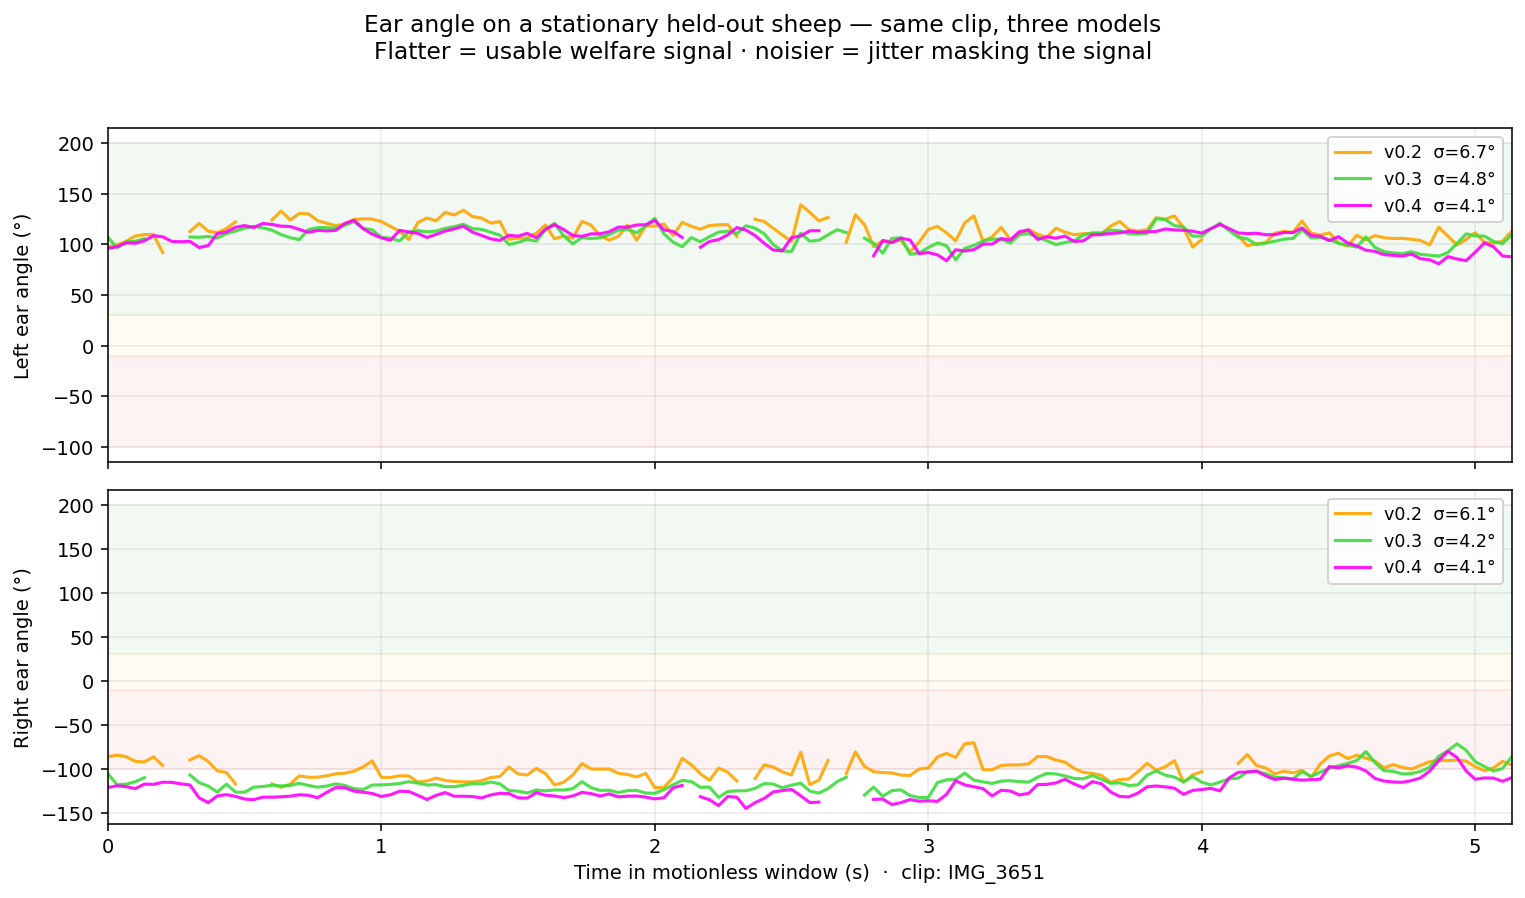
\includegraphics[width=0.92\textwidth]{earangle-img3651.png}
  \caption{Ear angle over the motionless window on HO-1 for v0.2, v0.3,
  v0.4, and v0.7. Flatter traces indicate a more stable measurement; noisier
  traces indicate keypoint jitter. The large v0.2$\rightarrow$v0.4 improvement is
  visible, while v0.7 overlaps v0.4 --- consistent with the post-v0.4 plateau
  (Table~\ref{tab:progression}). Legend $\sigma$ values are residual standard
  deviations. Shaded bands are the SPFES reference zones (green $\geq 30\dgr$,
  amber $-10\dgr$ to $30\dgr$, red $\leq -10\dgr$); they are literature reference
  bands, not diagnostic cutoffs.}
  \label{fig:earangle}
\end{figure}

\subsection{Training Progression and the v0.6 Regression}
\label{sec:progression}
Subsequent versions (v0.5--v0.7) continued the labeling flywheel, all
benchmarked on HO-1 (Table~\ref{tab:progression}). The monotonic
improvement of v0.2$\rightarrow$v0.4 does \emph{not} continue: from v0.4 onward
both the mean residual $\sigma$ and the ear-angle $\sigavg$ plateau near the
clip's noise floor. v0.5 reaches left $3.66\dgr$ / right $4.30\dgr$. v0.6 is a
mixed regression --- right ear $3.55\dgr$ (best recorded on HO-1) but left
ear $4.65\dgr$ (back to near-v0.2 levels) --- showing that per-keypoint labeling
consistency, not just instance count, drives stability. v0.7 recovers left to
$3.70\dgr$ (right $4.46\dgr$). Across all versions on HO-1, $\sigavg$
improves from $6.39\dgr$ (v0.2) to $4.08\dgr$ (v0.4, $-36\%$) and then oscillates
within ${\sim}0.1\dgr$ of $4.0\dgr$ --- a plateau, not continued improvement.

\begin{table}[t]
  \centering
  \caption{Full progression on HO-1. Improvement is monotonic only through
  v0.4; v0.5--v0.7 plateau, with v0.6 a per-keypoint regression.}
  \label{tab:progression}
  \begin{tabular}{lcccc}
    \toprule
    Version & Left ear $\sigma$ (\dgr) & Right ear $\sigma$ (\dgr) & $\sigavg$ (\dgr) & Residual $\sigma$ mean (px) \\
    \midrule
    v0.2 & 6.71 & 6.07 & 6.39 & 10.89 \\
    v0.3 & 4.82 & 4.21 & 4.52 & 8.90 \\
    v0.4 & 4.06 & 4.09 & 4.07 & 7.70 \\
    v0.5 & 3.66 & 4.30 & 3.98 & 7.83 \\
    v0.6 & 4.65 & 3.55 & 4.10 & 8.09 \\
    v0.7 & 3.70 & 4.46 & 4.08 & 7.90 \\
    \bottomrule
  \end{tabular}
\end{table}

\subsection{Statistical Robustness}
\label{sec:ci}
Each $\sigma$ above is a single point estimate from one ${\sim}5$\,s window on one
target sheep. To quantify within-window sampling uncertainty I computed
moving-block bootstrap 95\% confidence intervals (block $=10$ frames, 5000
resamples, on the detrended residual series; Table~\ref{tab:ci}). The intervals
are wide and adjacent-version intervals overlap almost completely: the gross
v0.2$\rightarrow$v0.4 improvement clears the band, but the
v0.4$\leftrightarrow$v0.7 differences do not. Two consequences follow, and the
paper's claims are calibrated to them. First, the training-scale signal is real
only at coarse resolution (roughly, 98 vs.\ 405 reviewed instances), not between
adjacent versions. Second, these intervals capture only within-window sampling;
they do \emph{not} capture the larger structural uncertainty of a single window,
single target sheep, and single clip per condition, which no resampling of one
window can estimate.

\begin{table}[t]
  \centering
  \caption{Moving-block bootstrap 95\% CIs on ear-angle residual $\sigma$
  (degrees). Adjacent-version intervals overlap; only the gross
  v0.2$\rightarrow$v0.4 change is separable.}
  \label{tab:ci}
  \begin{tabular}{llcc}
    \toprule
    Clip & Version & Left ear $\sigma$ (95\% CI) & Right ear $\sigma$ (95\% CI) \\
    \midrule
    HO-1 & v0.2 & 6.71 [5.56, 8.04] & 6.07 [4.65, 7.60] \\
    HO-1 & v0.4 & 4.06 [2.97, 4.99] & 4.09 [2.83, 5.26] \\
    HO-1 & v0.7 & 3.70 [2.96, 4.10] & 4.46 [3.08, 5.64] \\
    HO-2 & v0.2 & 5.37 [1.31, 8.82] & 2.24 [0.95, 3.09] \\
    HO-2 & v0.4 & 2.50 [1.15, 3.35] & 2.72 [1.22, 3.69] \\
    \bottomrule
  \end{tabular}
\end{table}

\subsection{v0.4 on Held-Out versus In-Distribution}
\label{sec:indist}
v0.4's held-out residual $\sigma$ of 7.70\,px approaches v0.3's in-distribution
numbers on its own training clips (4.10--5.92\,px, reported in the v0.3 benchmark
\citep{v03benchmark}). The ${\sim}1.8$--$3.6$\,px gap between in-distribution and
held-out performance is the generalization cost for an unseen scene; that this
gap is quantifiable at all was unavailable from the earlier within-distribution
benchmarks.

\subsection{Second Held-Out Clip: HO-2}
\label{sec:morning}
The second clip provides a cross-clip validation point, testing whether the
training-scale monotonicity observed on HO-1 (v0.2$\rightarrow$v0.4)
reproduces on an independently selected clip with different flock arrangement,
lighting, and target. Figure~\ref{fig:hero} shows the pipeline's multi-animal
output on this clip.

\subsubsection{Detection and Keypoint Stability}
Table~\ref{tab:morningheadline} reports results for v0.2--v0.4 plus the stock
baseline. The detection rate climbs from 88\% (v0.2) to 100\% (v0.4). Residual
$\sigma$ drops monotonically: $6.73 \rightarrow 4.22$ ($-37\%$) $\rightarrow 3.85$\,px
($-9\%$ from v0.3, $-43\%$ from v0.2) --- the same monotonic v0.2$\rightarrow$v0.4
pattern as HO-1. Raw $\sigma$ varies 41--58\,px, driven by lateral head
drift rather than model noise.

\begin{table}[t]
  \centering
  \caption{HO-2 held-out results. Stock-YOLO detection is the COCO-sheep-class
  rate (Section~\ref{sec:stock}); the any-class rate (100\%) is not reported as a
  detection figure because it does not reflect sheep localization.}
  \label{tab:morningheadline}
  \begin{tabular}{lcccc}
    \toprule
    Metric & Stock YOLO & v0.2 & v0.3 & v0.4 \\
    \midrule
    Sheep-class detection (full clip, 986 frames) & 118 (12\%) & 929 (94\%) & 986 (100\%) & 986 (100\%) \\
    In-ROI detection (window, 150 frames)         & 0 kpts     & 132 (88\%) & 149 (99\%) & 150 (100\%) \\
    Residual $\sigma$ (mean, 5 kpts, px)          & ---        & 6.73       & 4.22       & 3.85 \\
    Raw $\sigma$ (mean, 5 kpts, px)               & ---        & 41.53      & 56.09      & 58.35 \\
    \bottomrule
  \end{tabular}
\end{table}

\subsubsection{Per-Keypoint Residual $\sigma$}
Table~\ref{tab:morningperkpt} reports per-keypoint residual $\sigma$. The pattern
differs from HO-1: v0.2's largest variance is on the right ear (base
8.10\,px, tip 11.79\,px), while the left side and nose are already reasonably
stable at 98 instances. This asymmetry likely reflects the target's pose and the
morning lighting angle. By v0.3 the right-ear asymmetry largely resolves, and by
v0.4 left/right ear-base $\sigma$ are nearly identical (2.36 vs.\ 2.63\,px),
suggesting the model has learned symmetric ear placement from diverse views.
v0.4's ear-tip $\sigma$ of 4.38--5.69\,px on a 316-px-wide head is
${\sim}1.4$--$1.8\%$ of head width, versus $3.3$--$4.2\%$ on HO-1's
234-px-wide head; the larger apparent head (${\sim}1.35\times$) partly but not
fully explains the lower pixel $\sigma$.

\begin{table}[t]
  \centering
  \caption{Per-keypoint residual $\sigma$ (px) on HO-2.}
  \label{tab:morningperkpt}
  \begin{tabular}{lcccc}
    \toprule
    Keypoint & v0.2 & v0.3 & v0.4 & $\Delta$ v0.2$\rightarrow$v0.4 \\
    \midrule
    Nose           & 4.07  & 3.75 & 4.18 & $+3\%$ \\
    Left ear base  & 3.46  & 2.54 & 2.36 & $-32\%$ \\
    Right ear base & 8.10  & 2.91 & 2.63 & $-68\%$ \\
    Left ear tip   & 6.21  & 6.12 & 4.38 & $-29\%$ \\
    Right ear tip  & 11.79 & 5.79 & 5.69 & $-52\%$ \\
    \midrule
    \textbf{Mean}  & \textbf{6.73} & \textbf{4.22} & \textbf{3.85} & \textbf{$-43\%$} \\
    \bottomrule
  \end{tabular}
\end{table}

\subsubsection{Ear-Angle Stability}
Table~\ref{tab:morningearangle} reports ear-angle residual $\sigma$. On
HO-1 the left/right $\sigma$ were roughly symmetric; here v0.2 shows a
pronounced asymmetry ($5.37\dgr$ left vs.\ $2.24\dgr$ right) that resolves by v0.3
and re-emerges smaller in v0.4 and v0.7. This may reflect genuine anatomical
asymmetry in this sheep's ear carriage or a systematic left/right bias from the
viewing angle. v0.7's $\sigavg = 2.84\dgr$ is $7.1\%$ of the SPFES $40\dgr$ band.
Note that on this clip v0.4's $\sigavg$ is $2.61\dgr$ --- slightly lower than
v0.7's $2.84\dgr$; the two are within each other's bootstrap intervals
(Table~\ref{tab:ci}), so v0.7 is not an improvement over v0.4 here.

\begin{table}[t]
  \centering
  \caption{Ear-angle residual $\sigma$ (degrees) on HO-2.}
  \label{tab:morningearangle}
  \begin{tabular}{lcc}
    \toprule
    Version & Left ear $\sigma$ (\dgr) & Right ear $\sigma$ (\dgr) \\
    \midrule
    v0.2 & 5.37 & 2.24 \\
    v0.3 & 2.49 & 2.08 \\
    v0.4 & 2.50 & 2.72 \\
    v0.7 & 2.39 & 3.29 \\
    \bottomrule
  \end{tabular}
\end{table}

\subsubsection{Two-Clip Cross-Comparison}
\label{sec:crossclip}
Table~\ref{tab:crossclip} compares ear-angle $\sigavg$ across the two clips at
equivalent training scale. At identical scale (405 instances, 8 videos), v0.4
achieves $\sigavg = 4.08\dgr$ on HO-1 and $2.61\dgr$ on HO-2
--- a 36\% difference attributable to the clip, not the model. Three factors
likely contribute: the larger apparent head on HO-2
(${\sim}1.35\times$ wider) reduces pixel $\sigma$ for a fixed angular jitter; the
target is more isolated; and the morning lighting gives higher tan-on-green
contrast. This is precisely why the cross-clip number must not be read as a
version improvement: \textbf{the $2.84\dgr$ reached by v0.7 on HO-2
is a noise-floor measurement on an easier clip, and on matched clips v0.7 and
v0.4 are statistically indistinguishable} (Table~\ref{tab:ci}). A single
held-out clip provides a lower bound rather than a point estimate of model
performance; the two-clip comparison makes this explicit.

\begin{table}[t]
  \centering
  \caption{Cross-clip comparison of ear-angle $\sigavg$. The HO-1 vs.\
  HO-2 gap is a clip-difficulty effect, not a model improvement.}
  \label{tab:crossclip}
  \begin{tabular}{lccc}
    \toprule
    Metric & v0.4 on HO-1 & v0.4 on HO-2 & v0.7 on HO-2 \\
    \midrule
    Window size                       & 155 fr (5.2 s)        & 150 fr (5.0 s)        & 150 fr (5.0 s) \\
    Target head size (approx.)         & $234\times169$\,px     & $316\times185$\,px     & $316\times185$\,px \\
    Target type                        & Foreground dominant   & Background near fence & Background near fence \\
    Head centroid $\sigma$            & ${\sim}30$\,px ($x,y$) & 48\,px ($x$), 25 ($y$) & 48\,px ($x$), 25 ($y$) \\
    In-ROI detection rate              & 96\%                  & 100\%                 & 98.7\% \\
    Residual $\sigma$ (mean, px)      & 7.70                  & 3.85                  & --- \\
    $\sigma_{\text{left ear}}$ (\dgr)  & 4.06                  & 2.50                  & 2.39 \\
    $\sigma_{\text{right ear}}$ (\dgr) & 4.09                  & 2.72                  & 3.29 \\
    \textbf{$\sigavg$ (\dgr)}          & \textbf{4.08}         & \textbf{2.61}         & \textbf{2.84} \\
    $\sigavg$ as \% of SPFES $40\dgr$  & 10.2\%                & 6.5\%                 & 7.1\% \\
    Reviewed instances                 & 405                   & 405                   & 523 \\
    Training videos                    & 8                     & 8                     & 11 \\
    \bottomrule
  \end{tabular}
\end{table}

\section{Discussion}

\subsection{What the Numbers Mean}
The headline result --- ${\sim}4.08\dgr$ ear-angle $\sigavg$ on HO-1 (v0.4)
and ${\sim}2.84\dgr$ on HO-2 (v0.7) --- establishes a noise floor
for automated ear-angle measurement from ambient pasture video. Whether
$2.8$--$4.1\dgr$ is ``good enough'' depends entirely on the application. For
detecting gross ear-position changes (a sustained shift from $+30\dgr$ alert to
$-10\dgr$ down/back, a $40\dgr$ range), $4\dgr$ jitter is 10\% of the decision
range and unlikely to generate false positives. For subtle within-band changes
(a $5\dgr$ shift within the neutral zone), $4\dgr$ jitter would drown the signal.
The appropriate use is therefore coarse temporal patterns --- sustained
ear-position state changes over minutes, not frame-to-frame micro-movements. The
stock baseline is instructive: a practitioner using off-the-shelf models would
obtain exactly zero ear-angle data points. The keypoint head must be grown
against the target animals; there is no pretrained shortcut.

\subsection{Limitations}
The following limitations, drawn from the project's \texttt{VALIDATION.md}
contract, constrain any claim made on these results.

\paragraph{Single flock, single breed, single geography.} The dataset is
${\sim}5$ Katahdin hair-sheep ewes (plus lambs) on one homestead in Middletown,
Delaware. No claim transfers to other breeds (wool, horned, cropped or floppy
ears), geographies, or management conditions without independent validation.

\paragraph{Single operator, single camera.} One non-veterinarian operator
captured all video with one smartphone and performed all reviews. There is no
inter-annotator agreement, no independent ground truth, and no vet-validated
keypoint placement. Labeling consistency is measured only indirectly through the
training progression.

\paragraph{Point estimates, no significance on fine deltas.} Each $\sigma$ is a
single point estimate from one window on one sheep. As Section~\ref{sec:ci}
shows, adjacent-version differences fall within the within-window bootstrap
band; only the gross v0.2$\rightarrow$v0.4 change is separable. No version
ranking finer than that should be inferred, and the bootstrap does not address
single-clip/single-window structural uncertainty.

\paragraph{Two held-out clips, same flock.} The protocol uses two held-out clips
spanning different lighting and arrangements, but both are from the same flock,
pasture, and camera. A multi-clip ablation (3--5 clips from different sessions
and weather) would strengthen the generalization claim.

\paragraph{Ambient-vs-clinical gap.} The SPFES thresholds \citep{mclennan2019}
were validated in clinical pain conditions with trained veterinary observers.
Generalizing them to ambient pasture observation --- where sheep move their ears
for vigilance, social signaling, insect avoidance, and wind --- is an unresolved
scientific question. This instrument can extract ear angles; it cannot tell you
what they mean.

\paragraph{The measurement is not the diagnosis.} Ear angle is one geometric
feature. Welfare is a multi-dimensional construct requiring veterinary
assessment \citep{berckmans2014precision}; pain is a clinical determination
requiring multiple indicators. This pipeline measures one feature. It is not a
welfare instrument.

\subsection{Known Failure Modes}
\begin{itemize}
  \item \textbf{Dark fleece / low contrast.} SAM~3 segmentation degrades on
  black-faced sheep at dusk; the trained model inherits this from its
  light-fleeced-only training data.
  \item \textbf{Motion blur.} Handheld capture of moving sheep is the median
  case; heavy blur degrades segmentation and keypoint stability.
  \item \textbf{Extreme angles.} Best on frontal and three-quarter views;
  profile views and full ear occlusion reduce keypoint availability.
  \item \textbf{Occlusion.} In crowded frames the model may detect the wrong
  sheep or place keypoints on occluded anatomy.
  \item \textbf{Wool-covered ears.} Heavy fleece can obscure ear shape entirely;
  untested on wool breeds.
\end{itemize}

\subsection{What Validation Against Stress Events Would Require}
Turning this instrument into a welfare-relevant tool requires: documented stress
events with timestamps (hoof trimming, tagging, separation, transport);
continuous pre/post-event monitoring; a within-animal delta analysis; and a
pre-registered kill criterion. The project's \texttt{VALIDATION.md} specifies
that if fewer than 70\% of documented stress events show a measurable change in
ear-angle features, the welfare project terminates and the write-up of what
failed becomes the deliverable. This paper describes the measurement instrument;
that follow-up project would determine whether the measurements are
welfare-informative.

\subsection{Negative Results as Features}
This work deliberately publishes negative results. The stock baseline (zero
keypoints, 12--35\% sheep detection) establishes that off-the-shelf models are
not a viable shortcut. The v0.6 regression (right ear at all-time best $3.55\dgr$
but left ear regressing to $4.65\dgr$) demonstrates that more data does not
monotonically improve all keypoints; per-keypoint coverage and per-session
labeling consistency matter at least as much as instance count. The post-v0.4
plateau (Section~\ref{sec:progression}) is reported rather than hidden behind a
selectively quoted best version. And the v0.3 benchmark correction --- admitting
that the originally-claimed ``held-out'' clips were actually in v0.3's training
distribution --- is published alongside the corrected v0.4 benchmark
\citep{v03benchmark}. These are evidence that the measurement methodology is
working as designed.

\section{Conclusion}
I have presented SamSeesSheep, a measurement pipeline that converts ambient
pasture video into quantified ear-angle features using a foundation-model
annotation flywheel. The pipeline produces a small edge-runnable model (2.5\,M
parameters, ${\sim}10$\,MB) that places five keypoints on every detected sheep
head and achieves ear-angle residual $\sigavg$ of $4.08\dgr$ (v0.4 on HO-1)
and $2.84\dgr$ (v0.7 on HO-2) --- a metric literally unmeasurable
with off-the-shelf object detectors. The training progression shows monotonic
improvement in keypoint stability from 98 to 405 reviewed instances (v0.2 to
v0.4), then a plateau at the clip noise floor with a documented v0.6 regression;
the benchmark protocol, applied to two independent held-out clips with bootstrap
confidence intervals, provides a reproducible methodology for quantifying
measurement quality and its uncertainty.

I am explicit about the boundary: this is a measurement instrument, not a pain
detector or welfare scorer. It measures ear-angle features with quantified
stability. Whether those features are welfare-informative is a question for the
follow-up validation study this instrument is designed to enable. Future work
includes additional held-out clips spanning varied weather and camera positions;
cross-flock generalization on wool breeds and other geographies; validation
against documented stress events with the kill criterion above; inter-annotator
agreement measurement; and continuous-monitoring deployment at water troughs or
handling chutes, where sustained ear-position patterns become the unit of
measurement.

\section*{Data and Code Availability}
The code, benchmark scripts, machine-readable benchmark artifacts, paper source,
and documentation are available under the MIT License at
\url{https://github.com/antonemking/SamSeesSheep}. Reproducibility is layered, so
each headline number can be re-derived at the level a reader is equipped for.

\paragraph{In the repository (clone and verify).} Every $\sigma$, detection rate,
and per-keypoint number in this paper is stored in committed JSON artifacts under
\texttt{sheep-yolo/artifacts/} and is checkable in one command with
\texttt{sheep-yolo/scripts/verify\_paper\_claims.py}, which reads only those JSONs
and re-validates each value against the paper (44/44 checks pass on a fresh
clone). The bootstrap confidence intervals of Table~\ref{tab:ci} are in
\texttt{bench\_bootstrap\_ci.json}.

\paragraph{Companion artifacts (weights and cached predictions).} The trained
per-version weights (\texttt{sheep-pose-v0.\{2--7\}-yolo26n}) are gitignored for
size and published on the Hugging Face Hub at
\url{https://huggingface.co/antking1/sheep-pose-yolo26n}, with a
model card and a persistent DOI (\href{https://doi.org/10.57967/hf/9129}{10.57967/hf/9129})
pinned to a fixed revision. The per-frame model-prediction caches
(\texttt{sheep-yolo/artifacts/\_cache/*.pkl}, ${\sim}3$\,MB total) ship as an asset
on the \texttt{paper-artifacts-v0.7} GitHub release
(\url{https://github.com/antonemking/SamSeesSheep/releases/tag/paper-artifacts-v0.7}).
With the caches, every
committed benchmark JSON can be regenerated from scratch
(\texttt{gen\_bench\_Test\_Clip\_Morning.py} for HO-2; \texttt{gen\_residual\_px.py}
and the archived \texttt{bench\_v02\_v03.py} /
\texttt{bench\_v04\_v05\_v0\{6,7\}.py} for HO-1), and the ear-angle chart of
Figure~\ref{fig:earangle} with \texttt{gen\_ear\_angle\_chart.py}. The hero still
of Figure~\ref{fig:hero} is a frame from
\texttt{synced-lanes-6ewes-pro-Test\_Clip\_Morning.mp4}, also in the release.

\paragraph{Available on request (raw video and dataset).} The held-out clips
(HO-1, HO-2) and the full reviewed-keypoint training dataset are retained
off-repository for size and to limit redistribution of identifiable homestead
footage; they are available from the author on request. A reader with the raw
clips and the released weights can reproduce the cached predictions themselves;
a reader without them reproduces every published number from the caches onward.

\paragraph{Reported from outside the verification harness.} Three figures are
sourced outside the repository artifacts and are disclosed as such: the validation
mAP50-95 values (Table~\ref{tab:dataset}) come from the Ultralytics training logs
produced on the cloud GPU (only the weights, not the logs, return to the laptop);
the in-distribution $4.10$--$5.92$\,px residual-$\sigma$ range
(Section~\ref{sec:indist}) is quoted from the prior v0.3 benchmark
report~\citep{v03benchmark}, whose per-clip JSONs are training-set data held
off-repository; and the held-out clips were screened for low visual similarity to
the training videos at capture time and were never pushed to the labeler
(enforced by per-file checksum dedup) --- an author attestation the public
artifacts cannot independently re-derive.

\section*{Acknowledgments}
I thank the open-source computer-vision community whose tools made a
solo-operator pipeline feasible: Ultralytics for YOLO and YOLO-pose, and Meta AI
for the Segment Anything family, including SAM~3. I also thank the Katahdin ewes
of Middletown, Delaware, for their patience during repeated filming sessions.

\bibliographystyle{unsrtnat}
\bibliography{paper}

\appendix
\section*{Note on scope}
\emph{This work was conducted on a single Katahdin flock in Middletown,
Delaware, using one smartphone camera and one human reviewer (the author, who is
not a veterinarian). All claims are bounded by the scope described in the
project's \texttt{VALIDATION.md} contract. No pain detection. No welfare scoring.
A measurement instrument.}

\end{document}
